\chapter{Implementasi dan Pengujian}
\label{chap:implementasidanpengujian}

Bab ini akan membahas mengenai implementasi serta pengujian sistem perekaman ulang yang diterapkan dalam SharIF-Judge.

\section{Implementasi}
\label{sec:5:implementasi}

Bagian ini menjelaskan hasil implementasi sistem pemutaran ulang pada SharIF-Judge berdasarkan perancangan pada Bab \ref{chap:analisis}. Pada saat implementasi juga dilakukan penyesuaian pada peracangan yang sudah dibuat untuk mengatasi kendala yang dialami pada saat implementasi. 

\subsection{Merekam Peristiwa pada IDE}
\label{sub:5:2:merekam}

Fitur merekam peristiwa pada editor kode diimplementasikan untuk menangkap seluruh interaksi pengguna terhadap IDE dan SharIF-Judge pada saat pengguna menyelesaikan sebuah masalah dalam \textit{assignment}. Data yang direkam akan digunakan untuk memutar ulang penyelesaian yang dilakukan oleh pengguna. Fitur ini diimplementasikan dengan memanfaatkan \textit{Library Ace}, \textit{event hooks} pada \textit{JavaScript}. Implementasi ini akan memerlukan penyesuian pada bagian \textit{JavaScript} yaitu file \verb|assets/js/shj_submit.js| yang dimuat pada halaman \textit{Submit}.

Berikut merupakan alur sistem perekaman peristiwa:
\begin{enumerate}
    \item Inisialisasi Perekam \\
    Pada alur ini, semua perekaman akan diinisialisasi dengan menjalankan sebuah fungsi dinamakan \verb|recordStart|. Fungsi ini akan memanggil seluruh \textit{event hooks} dan \textit{event listener} dalam \textit{Library ace} agar dinyalakan. 
    
    Dalam menjalankan fungsi \textit{event listener}, dibutuhkan dua argumen yaitu event yang akan di panggil dan sebuah \textit{callback function} yang akan dieksekusi ketika \textit{event} tersebut terjadi. 
    
    Implementasi akan dibuat 2 objek \textit{JavaScript} yang menjadi fungsi \textit{event listener} yaitu objek pemanggilan \textit{event listener} dan objek menyimpan \textit{callback function} yang dipakai oleh \textit{event listener} masing-masing. Kode \ref{kode:5:1:objcallback} merupakan objek \textit{callback function} yang diimplementasikan.
    \begin{lstlisting}[caption={objek \textit{callback function}}, label={kode:5:1:objcallback}]
const handlers = {
    editor_change: (e) =>
        recordEvent(e.action, {
            data: e.lines,
            start: e.start,
            end: e.end,
        }),
        ...
}
    \end{lstlisting}
    
    Kode \ref{kode:5:1:objeventlist} merupakan objek pemanggilan \textit{event listener} yang dipanggil pada saat inisialisasi dan mendapatkan fungsi \textit{callback function} dari objek \textit{handlers} pada Kode \ref{kode:5:1:objcallback}.
    \begin{lstlisting}[caption={objek \textit{event listener}}, label={kode:5:1:objeventlist}]
const addListener = {
    editor_change: () => editor.session.on("change", handlers.editor_change),
    ...
}
    \end{lstlisting}

    Setelah itu objek \textit{addListener} akan dipanggil oleh fungsi \verb|recordStart|. Kode \ref{kode:5:1:eventlistener} menunjukkan fungsi yang dipanggil saat inisialisasi. 
    
    \begin{lstlisting}[caption={Beberapa \textit{event listener} yang dipanggil}, label={kode:5:1:eventlistener}]
addListener.editor_change();
    \end{lstlisting}
    
    Fungsi \verb|recordStart| akan dijalankan setiap kali pengguna mengubah \textit{problem} yang dipilih dalam halaman Submit untuk memulai rekaman peristiwa.

    \item Penyimpan sebuah rekaman \\
    Untuk setiap perekaman yang dibutuhkan, dijalankan sebuah fungsi yang mendeteksi perubahan tersebut dan menjalankan sebuah \textit{callback function} saat terjadi perubahan tersebut. Fungsi ini dipnaggil pada saat inisialisasi. \textit{Callback function} tersebut akan mendapatkan argumen sesuai dengan perubahan yang dideteksi. Pada contohnya untuk perubahan teks pada editor kode yaitu fungsi \verb|onchange|, argumen yang diberikan merupakan teks yang dimasukan yaitu contohnya adalah `A', dan juga posisi dimana teks tersebut dimasukkan dalam editor kode. Kode \ref{kode:5:1:argonchange} merupakan contoh argumen yang diberikan.
    \begin{lstlisting}[caption={Contoh argumen yang diberikan oleh fungsi onchange}, label={kode:5:1:argonchange}]
{
    data: ["A"], 
    start: {row: 0, column: 1}, 
    end:{ row: 0, column: 2}
}
    \end{lstlisting}
    Setelah itu data akan disimpan dalam sebuah objek \textit{JavaScript}
    seperti yang sudah dijelaskan pada Bab \ref{sec:4:2:storerekaman}. data argumen akan disimpan menggunakan key `args' atau `payload'.
    
    \item Penyimpanan data rekaman \\
    Selanjutnya sebuah \textit{event} atau rekaman yang sudah dicatat dan menjadi sebuah objek \textit{JavaScript} bernama \verb|recording|. seluruh event rekaman akan simpan dalam sebuah \textit{array} dalam \verb|recording| dengan key `events' seperti yang sudah dijelaskan pada Bab \ref{sec:4:2:storerekaman}. \verb|recording| juga memiliki waktu dimulainya rekaman, isi awal editor kode, posisi awal kursor dalam editor kode. \verb|recording| juga memiliki fungsi \verb|init| untuk meninisialisasi seluruh objek \verb|recording|.

    \begin{lstlisting}[caption={Contoh argumen yang diberikan oleh fungsi onchange}, label={kode:5:1:recordingobj}]
const recording = {
    events: [],
    startTime: -1,
    startValue: "",
    startSelection: [],

    init: () => {
        recording.events = [];
        recording.startTime = Date.now();
        recording.startValue = editor.getValue();
        recording.startSelection = getSelection(editor);
    },
};
    \end{lstlisting}

    Kode \ref{kode:5:1:recordingobj} merupakan \verb|recording| pada saat keadaan kosong. Pada objek \verb|recording|, \verb|events| merupakan sebuah array dengan isi sebuah rekaman event, \verb|startTime| merupakan waktu awal rekaman dimulai, \verb|startValue| merupakan isi awal dalam editor kode, dan \verb|startSelection| merupakan posisi awal kursor dalam editor kode.
\end{enumerate}

Berikut merupakan peristiwa yang akan direkam oleh sistem perekaman:
\begin{itemize}
    \item \verb|editor.change|: Peristiwa ini akan menangkap perubahan isi teks dalam editor kode.
    \item \verb|editor.changeCursor|: Peristiwa ini akan menangkap perubahan kursor dalam editor kode. 
    \item \verb|editor.changeSelection|: Peristiwa ini akan menangkap setiap perubahan yang terjadi pada \textit{selection} kursor dalam editor kode.
    \item \verb|window.focus|: Peristiwa ini akan menangkap pengguna \textit{focus} pada SharIF Judge web page. 
    \item \verb|window.blur|: Peristiwa ini akan menangkap pengguna pada saat pengguna tidak \textit{focus} pada SharIF Judge web page atau \textit{focus} pada aplikasi lain atau web page lain.
    \item \verb|window.visibilitychange|: Peristiwa ini akan menangkap pengguna yang mengubah \textit{tab} dari SharIF Judge ke \textit{tab} lain dalam browser.
    \item \verb|pdf_viewer.focusin|: Peristiwa ini akan menangkap pengguna pada saat pengguna \textit{focus} pada PDF Viewer dalam IDE.
    \item \verb|pdf_viewer.focusout|: Peristiwa ini akan menangkap pengguna pada saat pengguna tidak \textit{focus} pada PDF Viewer dalam IDE.
    \item \verb|editor_input.input|: Peristiwa ini akan menangkap perubahan isi editor input dalam IDE. 
    \item \verb|editor_output.change|: Peristiwa akan menangkap \textit{output} saat terjadinya aksi \textit{Execute}.
    \item \verb|save.click|: Peristiwa ini akan menangkap aksi \textit{Save} yang dilakukan pengguna.
    \item \verb|execute.click|: Peristiwa ini akan menangkap aksi \textit{Save \& Execute} yang dilakukan pengguna.
    \item \verb|submit.click|: Peristiwa ini akan menangkap aksi \textit{Save \& Submit} yang dilakukan pengguna.
\end{itemize}

Seluruh alur sistem perekaman peristiwa dalam SharIF-Judge akan ditambahkan ke dalam file \verb|assets/js/|\verb|shj_submit.js|. Kode perubahan terdapat pada Lampiran \ref{lamp:A}.

\subsubsection{Perbaikan Implementasi}

Pada saat mengujian fungsi penyimpanan rekaman, dalam tahap alur penyimpanan data rekaman dan juga bagaimana inisialisasi perekaman akan diubah dari perancangan Bab \ref{sub:4:3:merekam}. Hal ini dikarenakan saat pengguna memilih ulang masalah atau memuat ulang halaman Submit, maka semua events yang sudah direkam akan hilang. Maka dari itu berikut merupakan perubahan pada alur fitur sistem perekaman ketikan:

\begin{enumerate}
    \item Inisialisasi Perekam \\
    Alur inisialisasi akan diubah agar dapat memuat events yang sebelumnya sudah disimpan dalam objek \textit{JavaScript} bernama \verb|befRecording|. Oleh karena itu, dibutuhkannya penambahan fungsi pada \textit{Controller} \verb|Submit.php| yaitu fungsi untuk mengambil data rekaman sebelumnya bernama \verb|load_rec| yang mengambil argumen pengenal masalah yang dipilih oleh pengguna. Kode penambahan terdapat di Lampiran \ref{lamp:A}

    \item Penyimpan data rekaman \\
    Pada objek \verb|recording|, \verb|startValue| dan \verb|startSelection| tidak dibutuhkan karena isi awal dari editor kode dan juga posisi awal kursor dalam editor kode akan selalu berisi dengan nilai kosong yaitu teks kosong dan posisi di baris dan kolom pertama.
\end{enumerate}

\subsection{Menyimpan Rekaman pada Sistem}
\label{sub:5:2:storerekaman}

Fitur penyimpanan rekaman pada sistem bertujuan untuk menyimpan data secara permanen ke dalam database dan \textit{server} agar dapat diputar kembali di lain waktu. Berikut merupakan alur fitur penyimpanan rekaman pada sistem:

\begin{enumerate}
    \item Mengirimkan Data ke \textit{Server} \\
    Dalam halaman Submit, pengguna memiliki 3 aksi penting dalam IDE SharIF-Judge yaitu: \textit{save}, \textit{execute}, dan \textit{submit}. Alur ini akan mengirimkan data rekaman pada saat pengguna melakukan aksi tersebut. Data yang dikirim merupakan objek \verb|recording| yang sudah jadikan sebagai teks JSON dengan menggunakan fungsi \verb|JSON.stringify|.

    \item Menyimpan Data Dalam File Sistem \\
    File akan disimpan dalam direktori yang sama dengan penyimpanan kode \textit{submission} yang dijelaskan pada Bagian \ref{sub:3:1:penyimpanankode}. File akan diisi secara langsung oleh data rekaman dan tidak diubah oleh \textit{server}. Penamaan file dapat dibagi berdasarkan aksi yang membuat pengguna mengirimkan data rekaman. Untuk aksi \textit{save} dan \textit{execute}, file dengan data rekaman akan disimpan dengan nama \verb|recording|. Untuk aksi \textit{submit}, file akan disimpan dengan nama \verb|recording| dilanjutkan dengan sebuah `-' dan \textit{submit id} yang dibuat. File tersebut memiliki tipe data yang sama yaitu JSON karena itu extensi file yang digunakan adalah \verb|.json|.
 
    \item Menyimpan Data Dalam Database \\
    Saat penyimpanan data ke dalam file sistem berhasil, maka penyimpanan kedalam database juga akan dilakukan. Data yang akan disimpan kedalam database akan digunakan untuk mendaftar rekaman yang ada dalam sistem, maka data yang akan disimpan bukan data rekaman melainkan data statistik. Berikut merupakan data yang akan disimpan ke dalam Database:
    \begin{itemize}
        \item \verb|rec_id|: pengenal rekaman yang sama dengan \textit{submit id}.  
        \item \verb|username|: nama pengguna yang mengirimkan data rekaman.
        \item \verb|problem_id|: pengenal masalah yang pengguna kerjakan.
        \item \verb|assignment_id|: pengenal tugas yang pengguna kerjakan.
        \item \verb|upload_at|: waktu sistem penyimpan data rekaman.
    \end{itemize}
    Untuk membuat databasenya sendiri, dibutuhkan penambahan tabel bernama tabel \verb|recording| yang memiliki lima atribut di atas. Kode \ref{kode:5:2:adddatabasetable} menunjukkan pembuatan tabel baru menggunakan \textit{CodeIgniter} dalam SharIF-Judge.

    \begin{lstlisting}[caption={Kode membuat database pada SharIF-Judge}, label={kode:5:2:adddatabasetable}]
// create table 'recording'
$fields = array(
    'rec_id' 	    => array('type' => 'INT', 'constraint' => 11, 'unsigned' => TRUE),	
    'upload_at'		=> array('type' => $DATETIME),
    'assignment' 	=> array('type' => 'SMALLINT', 'constraint' => 4, 'unsigned' => TRUE),
    'problem'       => array('type' => 'SMALLINT', 'constraint' => 4, 'unsigned' => TRUE),
    'username'      => array('type' => 'VARCHAR', 'constraint' => 20),
);
$this->dbforge->add_field($fields);
if (! $this->dbforge->create_table('recording', TRUE))
    show_error("Error creating database table " . $this->db->dbprefix('recording'));
// ADD Unique constraint
$this->db->query(
    "ALTER TABLE {$this->db->dbprefix('recording')}
        ADD CONSTRAINT {$this->db->dbprefix('sruap_unique')} UNIQUE (rec_id, username, assignment, problem);"
);
    \end{lstlisting}

    Mengikuti arsitektural \textit{CodeIgniter}, untuk menambahkan sebuah data ke dalam database perlu menggunakan sebuah \textit{Model}. Oleh karena itu, dibutuhkannya \textit{model} baru bernama \verb|Recording_model.php| yang ditambahkan fungsi \verb|add_recording()| yang memiliki argumen yaitu seluruh data yang ingin disimpan dalam database.

    Untuk aksi \textit{save} dan \textit{execute} dimana tidak adanya \textit{submit id} maka akan menjadi angka nol (`0') pada pengenal rekamannya atau \verb|rec_id| jika aksinya merupakan \textit{submit}.
\end{enumerate}

Untuk alur pengiriman data ke \textit{server}, dibutuhkannya penambahan kode ke dalam \verb|assets/js/|\\\verb|shj_submit.js|. Agar dapat menyimpan dibutuhkannya perubahan dalam kode \textit{Controller} \verb|Submit| pada fungsi \verb|save($type)| dan fungsi \verb|_submit()|. Kode pembahan terdapat pada Lampiran \ref{lamp:A}.

\subsubsection{Perbaikan Implementasi}

Pada pengujian yang sama dengan Bab \ref{sub:5:2:merekam}, dibutuhkannya perubahan pada alur pengirimkan data ke server. Karena \textit{events} yang sudah di save dapat terhapus karena pengguna memilih ulang masalah dan memuat ulang halaman Submit, yang membuat rekaman inisialisasi dan menghapus rekaman lama. Maka pada saat mengirimkan data \verb|recording|, akan disertakan juga data \verb|befRecording| yang sudah diambil pada saat inisialisasi. Format pengiriman data juga akan berubah dikarenakan adanya rekaman yang lama menjadi sebuah \textit{key} dan \textit{value} karena hanya dua value yang harus disimpan yaitu \textit{events} sebagai \textit{value} dan \textit{startTime} sebagai \textit{key}. Maka format ini menjadi format keseluruhan events yang terjadi dan dapat disatukan dengan format yang sama menggunakan \textit{spread operator} agar seluruh rekaman lama digabungkan. Kode \ref{kode:5:2:mergedata} merupakan kode untuk mengirimkan teks JSON dengan mengabungkan kedua rekaman menggunakan \textit{spread operator}.

\begin{lstlisting}[caption={objek \textit{callback function}}, label={kode:5:2:mergedata}]
JSON.stringify({
    ...befRecording,
    [recording.startTime]: recording.events
}),
\end{lstlisting}

\subsection{Melihat Daftar Rekaman}

Fitur ini digunakan untuk melihat daftar rekaman mahasiswa yang tersimpan dalam sistem, pengguna juga dapat melihat isi rekaman yang terdapat dalam daftar rekaman tersebut. Fitur ini dibutuhkan dua tahap untuk diimplementasikan yaitu sebagai berikut:

\begin{itemize}
    \item Pengambilan Data Rekaman \\
    Fitur pengambilan data rekaman digunakan agar bagian depan SharIF-Judge dapat meminta daftar rekaman yang ada pada bagian belakang SharIF-Judge. Oleh karena ini merupakan sebuah halaman baru dalam SharIF-Judge, maka dibutuhkannya sebuah \textit{Controller} baru bernama \verb|Recording.php| yang menampilkan sebuah halaman baru yang dapat diakses melalui rute \verb|/recording/all/| yang menggunakan fungsi baru dalam \verb|Recording_model.php| yaitu fungsi untuk mendapatkan daftar rekaman dinamakan \verb|all_user_recordings|. Kode pertambahan pada \textit{Model} \verb|Recording.php| berada pada Lampiran \ref{lamp:A}.

    Berikut fungsi yang akan diimplementasikan dalam \textit{Controller} \verb|Recording.php|:
    \begin{enumerate}
        \item \verb|__construct()| \\
        Fungsi ini akan memuat seluruh kebutuhan \textit{Model} dan \textit{Helper} ke dalam \verb|Recording.php|, fungsi \textit{construct} juga akan membatasi akses oleh pengguna dibawah \textit{instructor}. Fungsi ini juga mendapatkan \textit{params url} yang dikirim oleh pengguna. 

        \item \verb|all()| \\
        Fungsi ini akan mengambil beberapa data yang dibutuhkan oleh antarmuka SharIF-Judge yaitu \textit{assignment} yang dipilih oleh pengguna menggunakan \verb|assignment_model|, \textit{problem} yang ada dalam \textit{assignment} tersebut menggunakan \verb|assignment_model|, dan daftar \textit{recording} yang tersimpan dalam sistem menggunakan \verb|recording_model|. Setelah itu, server akan menempatkan seluruh data tersebut ke dalam \textit{view} baru bernama \verb|recording_list.twig| untuk ditampilkan kepada pengguna.
    \end{enumerate}

    Seluruh alur untuk mengimplementasikan fitur pengambilan data rekaman dalam \textit{Controller} \verb|Recording.php| terdapat dalam Lampiran \ref{lamp:A}.

    \item Antarmuka dan Tampilan Data \\
    Antarmuka yang diimplementasikan akan dibuat serupa dengan perancangan pada Bab \ref{sub:4:1:pemutaranulang} yang diimplementasikan ke dalam SharIF-Judge. Data yang dikirim oleh \textit{Controller} \verb|Recording.php| juga dapat ditampilkan menggunakan \textit{Library twig} tanpa menbutuhkan \textit{JavaScript} maupun \textit{php} dalam antarmukanya. Gambar \ref{fig:hasil:recording_list} menunjukkan implementasi antarmuka beserta data yang terdapat dalam sistem. Untuk kode keseluruhan antarmuka menggunakan \textit{Library twig} dapat dilihat pada Lampiran \ref{lamp:A}.
\end{itemize}


\subsubsection{Perbaikan Implementasi}

Untuk fitur ini, tidak dilakukan perubahan pada implementasi yang sudah ada karena dianggap sudah memenuhi kebutuhan pengguna.

\subsection{Pemutaran Ulang Rekaman}

Fungsi pemutaran ulang rekaman menggunakan data rekaman yang sudah disimpan dalam sistem untuk memvisualisasikan proses penyelesaian masalah pengguna secara kronologis. Fitur pemutaran ulang ini membutuhkan yaitu sebagai berikut:

\begin{itemize}
    \item {Implementasi Antarmuka} \\
    Untuk menambahkan sebuah halaman baru dalam SharIF-Judge dibutuhkannya juga fungsi baru pada \textit{Controller} \verb|Recording.php|. Fungsi baru akan dinamakan \verb|index| untuk menampilkan sebuah \textit{view} baru bernama \verb|recording.twig|. Fungsi \verb|index| akan menampilkan halaman baru itu melalui rute \verb|/recording/|. Penamaan \textit{index} itu agar rute tidak memerlukan \verb|/index| pada akhir rute karena jika rute \textit{function} (Bab \ref{sub:2:2:codeigniterurls}) akan otomatis mengarah pada fungsi \verb|index| dalam kelas tersebut.

    Fungsi \verb|index| akan mengirim data daftar rekaman pengguna lainnya dalam masalah yang dipilih. Data tersebut akan dipakai oleh \verb|recording.twig| untuk menambahkan daftar rekaman pengguna lainnya pada \textit{assignment} dan \textit{problem} yang sama. Gambar \ref{fig:hasil:recording} merupakan antarmuka yang diimplementasikan serupa dengan perancangan pada Bab \ref{sub:4:1:pemutaranulang}.

    \item Implementasi Memuat Data Rekaman \\
    \label{ssub:5:2:4:memuatdata}Data rekaman yang akan diambil sudah disimpan (Bab \ref{sub:5:2:storerekaman}) dalam sistem. Tetapi data rekaman tidak akan dikirim oleh \textit{Controller} pada saat halaman \textit{recording} dimuat, melainkan menggunakan AJAX pada halaman \textit{recording}. Maka dibutuhkannya fungsi baru pada \textit{Controller} \verb|Recording.php| dan sebuah assets \textit{JavaScript} baru bernama \verb|shj_function.js|.

    Fungsi baru dalam \textit{Controller} \verb|Recording.php| akan dinamakan \verb|download_record| yang memiliki argumen \verb|assignment_id|, \verb|problem_id|, dan \verb|rec_id|. Fungsi tersebut akan mengambil \textit{file} rekaman dalam file sistem dengan menggunakan argumen untuk mendapatkan lokasi dan nama \textit{file} rekaman (Bab \ref{sec:4:2:storerekaman}) SharIF-Judge dan mengirimkan file tersebut secara langsung. File juga akan dirikim dengan header \verb|Content-Type: application/json| dan \verb|Content-Disposition: attachment; filename=|\verb|"rec.json"|.

    Fungsi \verb|download_record| dipanggil pada saat halaman \textit{recording} dimuat dan \textit{JavaScript} \verb|shj_function.js| dengan fungsi baru yaitu \verb|getRecording|. Fungsi \verb|getRecording| akan meninisialisasi editor kode dalam antarmuka, mendapatkan data rekaman melalui fungsi \verb|download_record|, dan menformat data rekaman agar lebih mudah untuk di putar ulang. Berikut merupakan format data tambahan yang akan diubah oleh fungsi \verb|getRecording|:

    \begin{itemize}
        \item \verb|events|: Data rekaman
        \item \verb|eventsIndex|: sebuah map dengan \textit{key} waktu saat sebuah \textit{events} terjadi dan \textit{value index} waktu saat sebuah \textit{events} terjadi.
        \item \verb|indexEvents|: sebuah map dengan \textit{key index} waktu saat sebuah \textit{events} terjadi dan \textit{value} waktu saat sebuah \textit{events} terjadi.
        \item \verb|presumIndexDuration|: menkalkulasikan panjang rekaman sebelum rekaman selesai.
        \item \verb|length|: panjang data rekaman
        \item \verb|duration|: durasi dari seluruh rekaman yang ada pada data rekaman
    \end{itemize}

    Data akan disimpan dalam sebuah objek \textit{JavaScript} dinamakan \verb|recording| dan akan dipakai pada saat menjalankan rekaman dan untuk menampilkan histogram \textit{events} yang terjadi.

    \item Implementasi Menjalankan Rekaman \\
    Fitur menjalankan rekaman akan menggunakan data bedasarkan data yang didapatkan oleh AJAX yang dijelaskan pada bagian \ref{ssub:5:2:4:memuatdata}. Fitur menjalankan rekaman akan membutuhkan penambahan kode pada \textit{JavaScript} \verb|shj_function.js| yang akan menjalankan fungsi \verb|play| atau \verb|stop| untuk menjalankan atau memberhentikan rekaman oleh pengguna. 

    Fungsi menjalankan atau mematikan rekaman dibagi menjadi dua yaitu fungsi rekaman dalam IDE dengan data rekaman dinamakan \verb|Recording| dan fungsi timer yang digunakan untuk memberitahu kepada pengguna progress waktu pemutaran rekaman dinamakan \verb|Timer|.
    Fungsi \verb|Recording| menggunakan fungsi dalam \textit{Library Ace} dan fungsi \textit{JavaScript} untuk memperbaharui IDE antarmuka berdasarkan \textit{event} yang dipanggil, fungsi \verb|setTimeout| dalam \textit{JavaScript} akan digunakan untuk menjalankan \textit{event} selanjutnya bedasarkan perbedaan waktu antara event sekarang dan event selanjutnya dengan memanggil fungsi \verb|playRecording| dengan \textit{event} selanjutnya. Sedangkan fungsi \verb|Timer| menggunakan fungsi \verb|setInterval| yang akan dijalankan berulang untuk setiap detiknya dan memperbaharui progress waktu dalam antarmuka berdasarkan waktu yang sudah lewat.

    \item Menampilkan Histogram Events yang Terjadi \\
    Pada fungsi \verb|getRecording| setelah memuat data rekaman dan menformat data rekaman tersebut, fungsi \verb|setUpChart| akan dipanggil dan membuat data grafik histogram. Data histogram akan dimuat menggunakan \textit{Library} \verb|Chart.js|.

\end{itemize}

\subsubsection{Perbaikan Implementasi}

Untuk fitur ini, tidak dilakukan perubahan pada implementasi yang sudah ada karena dianggap sudah memenuhi kebutuhan pengguna.

\section{Pengujian Fungsional}
\label{sec:5:fungsional}

Pengujian fungsional dilakukan secara lokal. Berikut merupakan pengujian terhadap fitur-fitur sistem pemutaran ulang dalam SharIF Judge:

\begin{table}[H]
	\centering
	\caption{Tabel Pengujian Fungsional}
	\begin{tabular}{|p{0.5cm}| p{5.5cm}| p{6cm}| p{2.5cm}|} \hline
	No.	& Aksi Pengguna	& Reaksi yang diharapkan & Reaksi \\ \hline
	1 	& Memilih masalah dalam Halam Submit & Sistem memulai rekaman &	sesuai	\\ \hline
	2 	& Melakukan Aksi \textit{Save} & Menyimpan rekaman sesi dalam sistem & sesuai	\\ \hline
	3 	& Melakukan Aksi \textit{Save \& Execute} & Menyimpan rekaman sesi dalam sistem & sesuai	\\ \hline
	4 	& Melakukan Aksi \textit{Save \& Submit} & Menyimpan rekaman sesi dalam sistem & sesuai	\\ \hline
	5 	& Membuka Halaman Daftar Rekaman & Daftar Rekaman ditampilkan & sesuai	\\ \hline
	6 	& Memilih Rekaman dalam Halaman Rekaman & Memuka halaman Rekaman & sesuai	\\ \hline
	7 	& Menyaring Daftar Rekaman dengan User & Daftar rekaman menampilkan hanya daftar rekaman user & sesuai	\\ \hline
	8 	& Menyaring Daftar Rekaman dengan Problem & Daftar rekaman menampilkan hanya daftar rekaman untuk problem saringan & sesuai	\\ \hline
	9 	& Menyaring Daftar Rekaman dengan User dan Problem & Daftar rekaman menampilkan hanya daftar rekaman user pada problem saringan & sesuai	\\ \hline
	10 	& Membuka Halaman Rekaman & Rekaman ditampilkan & sesuai	\\ \hline
	11 	& Menjalankan Rekaman & Rekaman diputar ulang & sesuai	\\ \hline
	12 	& Memberhetikan Rekaman yang berjalan & Putaran ulang rekaman berhenti & sesuai	\\ \hline

	\end{tabular}
	\label{table:fungsional}
\end{table}

\section{Pengujian Eksperimental}
\label{sec:5:eksperimental}

Pada Bagian ini dilakukannya pengujian terhadap sistem Perekaman Ulang pada SharIF Judge.

\subsection{Lingkungan pengujian}
Pengujian sistem perekaman ulang akan dilakukan pada sebuah server VPS atau \textit{Virtual Private Server}. Pada server akan dijalankannya \textit{docker} agar sistem aplikasi akan identik dengan pada saat sistem sedang diimplementasikan. Kode \ref{kode:5:3:1:dockercompose} dan Kode \ref{kode:5:3:1:dockerfile} merupakan file \textit{docker-compose} dan \textit{Dockerfile} yang digunakan membangun sistem SharIF Judge dalam server VPS.

Tabel \ref{tab:5:1:keraspembangunan} menunjukkan spesifikasi perangkat keras yang digunakan saat pengujian.
\begin{table}[H]
    \caption{Perangkat Keras Lingkungan Pembangunan}
    \label{tab:5:1:keraspembangunan}
    \centering
    \begin{tabular}{|l|l|}
        \hline
        \textbf{Parameter}                  & \textbf{Nilai}              \\ \hline
        \textit{Processor}                  & \textit{AMD EPYC 9354P 2 vCPU} \\ \hline
        \textit{Random Access Memory (RAM)} & 8 GB                       \\ \hline
        \textit{Storage}                    & 100 GB \textit{SSD}           \\ \hline
    \end{tabular}
\end{table}

Tabel \ref{tab:5:2:1:lunakpembangunan} menunjukkan spesifikasi perangkat lunak yang digunakan saat pengujian.

\begin{table}[H]
    \caption{Perangkat Lunak Lingkungan Pembangunan}
    \label{tab:5:2:1:lunakpembangunan}
    \centering
    \begin{tabular}{|l|l|}
        \hline
        \textbf{Parameter}        & \textbf{Nilai}                                            \\ \hline
        Sistem Operasi            & \textit{Debian Version} 12     \\ \hline
        Bahasa Pemrograman        & PHP, \textit{JavaScript}, \textit{CSS}, dan \textit{HTML} \\ \hline
        \textit{Framework}        & \textit{CodeIgniter} 3.1.13                               \\ \hline
        \textit{Code Editor}      & \textit{Visual Studio Code} 1.99.3                        \\ \hline
        Perangkat Lunak Pendukung & \textit{Docker Version} 20.10.24+dfsg1                            \\ & \textit{Debian} 11-slim \\ & \textit{MySQL} 5.7 \\ & \textit{phpMyAdmin} 5.2.1 \\ & PHP 7.3.33\\ \hline
    \end{tabular}
\end{table}

\subsection{Eksperimen}

Pengujian dilakukan untuk mengetahui permasalah yang terjadi jika IDE dalam SharIF Judge dimasukkan sistem perekaman. Hasil Pengujian juga akan dianalisis secara sederhana agar dapat dibuatnya sebuah sistem untuk mendeteksi tindakan kecurangan.

Pengujian pada sistem pemutaran ulang dilakukan dengan mengajak beberapa peserta yang masih menempuh kuliah dan sudah lulus kuliah dengan mengerjakan tiga permasalahan dengan tingkat kesusahan mudah, sedang, dan sulit dalam waktu satu hari. Para peserta dianjurkan mengerjakan 2 soal yang sudah disediakan dan dapat melihat \textit{syntax} bahasa pemrograman. Pada pengujian peserta juga dapat melakukan kecurangan pada satu nomor dengan cara apapun. Kecurangan akan dianggap terjadi pada saat peserta melihat cara pengerjaan permasalah.

Berikut merupakan masalah yang ditemukan pada saat pengujian sistem pemutaran ulang:

\begin{itemize}
    \item Fitur menampilkan soal pada IDE \\
    Fitur ini tidak dapat dilakukan karena permasalahan dengan \textit{networking} dalam server VPS yang menjadikan tidak bisanya mengakses PDF permasalah dalam SharIF Judge dan menghasilkan \textit{status} 404. Fitur ini diabaikan karena fitur ini tidak mengganggu pengujian yang sedang berjalan, tetapi untuk peserta melihat soal dengan cara mendownload soal dan melihatnya pada aplikasi lain yang akan berdampak pada analisis hasil eksperimen.
    \item Fitur Menyimpan Rekaman pada Sistem \\
    Fitur ini tidak mengubah database pada saat pengguna melakukan aksi \textit{submit}. Pada saat aksi \textit{submit} dilakukan \textit{file} rekaman dibuah menjadi \textit{file} rekaman yang sudah di-\textit{submit} tetapi pada daftar rekaman dalam database itu sendiri belum dihapus dan pada saat rekaman di ambil, tidak ditemukannya rekaman tersebut dan mengembalikan error pada pengguna. Untuk menyelesaikan masalah ini, diperlukan sebuah fungsi baru dalam \textit{Model} \verb|Recording_model|. Kode \ref{kode:5:2:2:recording_model} merupakan fungsi yang ditambahkan pada \textit{Model} \verb|Recording_model|. 

    \begin{lstlisting}[language=php, caption={Fungsi tambahan pada \textit{Recording model}}, label=kode:5:2:2:recording_model]
public function remove_saveonly_recording($assignment_id, $problem_id, $username) {
    $this->db->delete('recording', array(
        'assignment' => $assignment_id, 
        'problem'=>$problem_id, 
        'username'=>$username, 
        'rec_id'=>0)
    );
}
    \end{lstlisting}

    Fungsi ini akan digunakan pada \textit{Controller} \verb|Recording| pada saat fungsi \verb|_submit()| dipanggil.

\end{itemize}

Setelah pengujian berakhir, peserta diminta untuk mengisi beberapa pertanyaan mengenai permasalahan yang dikerjakan dan juga beberapa pertanyaan mengenai pengalaman mengerjakan permasalah pemrograman. Tetapi karena tidak ada eksperimen untuk fitur melihat perekaman, tidak ada umpan balik untuk fitur melihat rekaman. 

\subsubsection{analisis Hasil Pengujian}
analisis ini dilakukan dengan melihat data yang rekaman yang sudah di proses dan menjadi bagan histogram dalam sistem dan bagan lainnya yang dibutuhkan pada proses analisis. Ada beberapa pola yang dapat dilihat pada saat melihat histogram hasil rekaman peserta pengujian. Berikut merupakan pola yang dapat dilihat pada:

\begin{itemize}
    \item Pola Pergantian Kode \\
    Pola ini dapat dilihat pada \textit{events} \verb|editor.change| dan hasil kode yang dibuat. Pola ini didasari dengan adanya \textit{Code Churn} atau bisa disebut dengan pengerjaan ulang kode. \textit{Code Churn} ini terjadi pada saat peserta atau mahasiswa menghapus atau menulis ulang kode program~\cite{hatica:churn}. Pada \textit{Code Churn} ada yang dinamakan \textit{Code Churn Rate} adalah sebuah tingkat pergantian kode selama sedang mengerjakan kode program tersebut. \textit{Code Churn Rate} dapat menilai seberapa banyak kode berubah dalam suatu tim, module, file maupun fungsi. Pada pola ini digunakannya \textit{Code Churn Rate} dalam tingkat file sebagai sebuah penilaian yang dapat dilakukan dengan menggunakan rumus sebagai berikut:
    
    \begin{center}
        \verb|(inserted_kode + removed_kode) / total_kode|
    \end{center}

    \verb|inserted_kode| dihutung dengan menjumlahkan total karakter yang di masukkan dalam editor. Begitu juga dengan \verb|removed_kode| dihitung dengan menjumlahkan total karakter yang dihapus dalam editor. \verb|total_kode| dihitung dengan menjumlahkan jumlah total karkater pada hasil kode program akhir. Berikut contoh perhitungan untuk \textit{Code Churn Rate}:

    \begin{figure}[H]
        \centering
        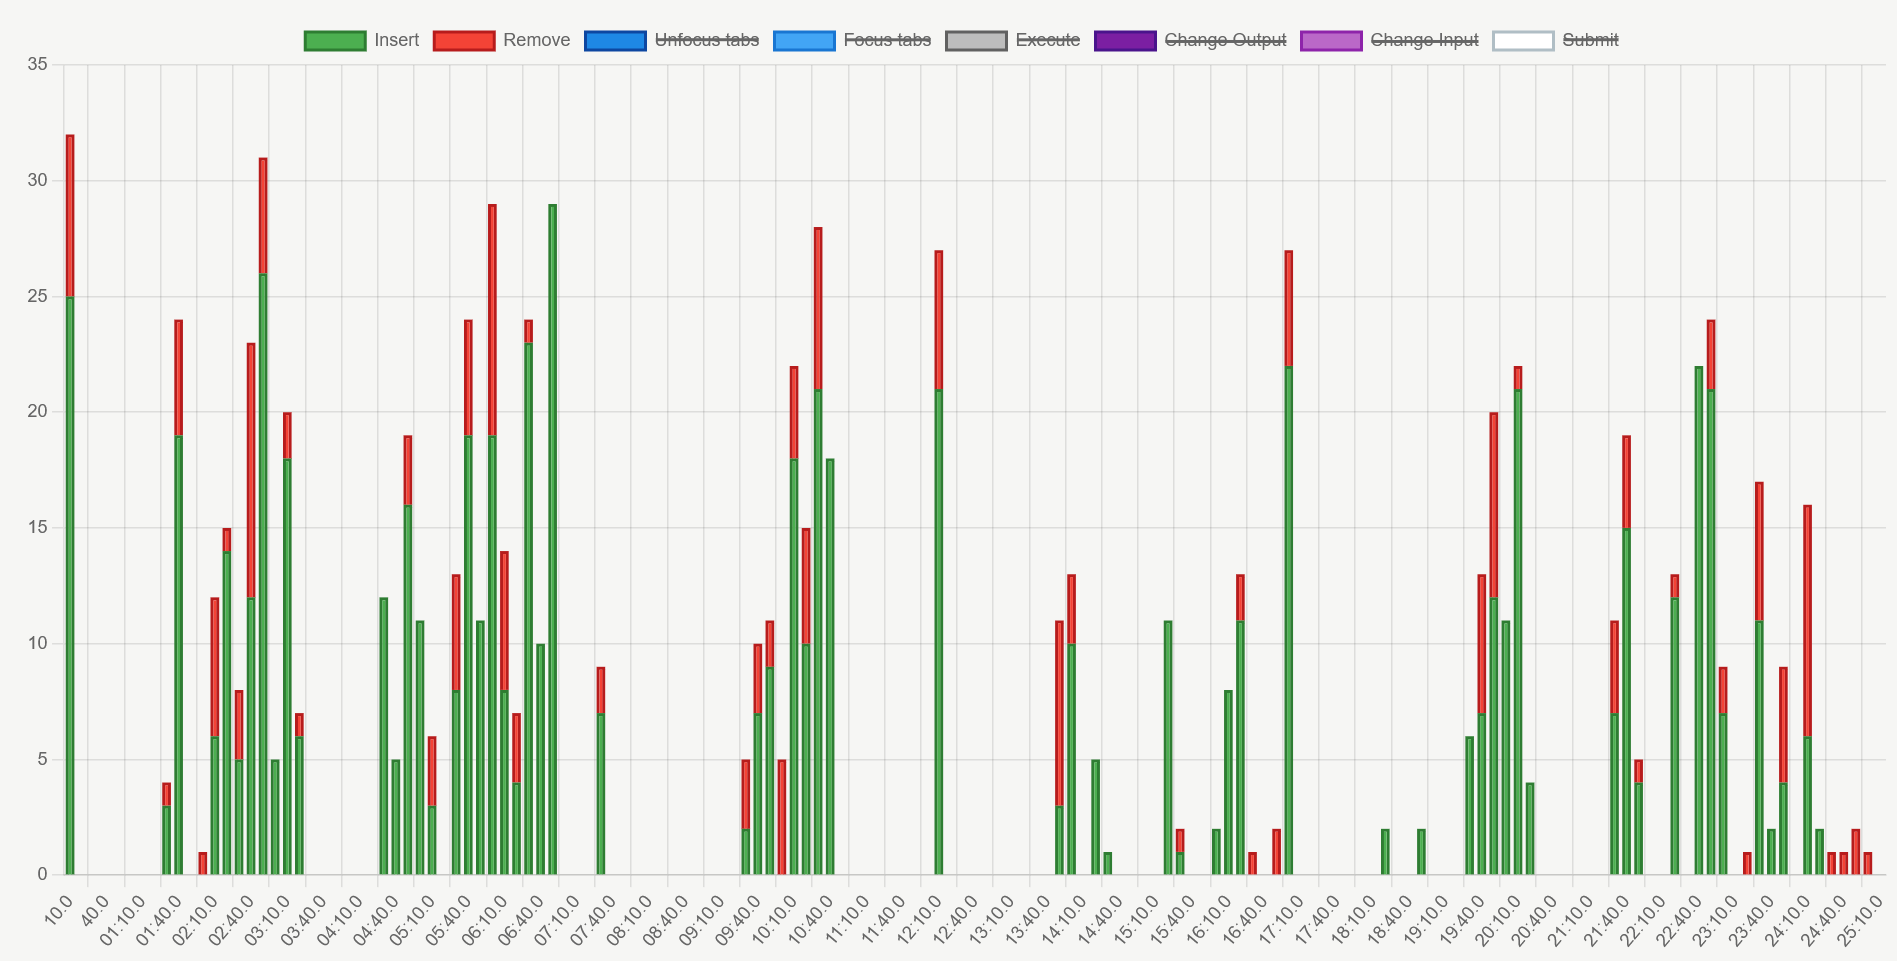
\includegraphics[width=0.49\textwidth]{experiment/insert-many-rework.png}
        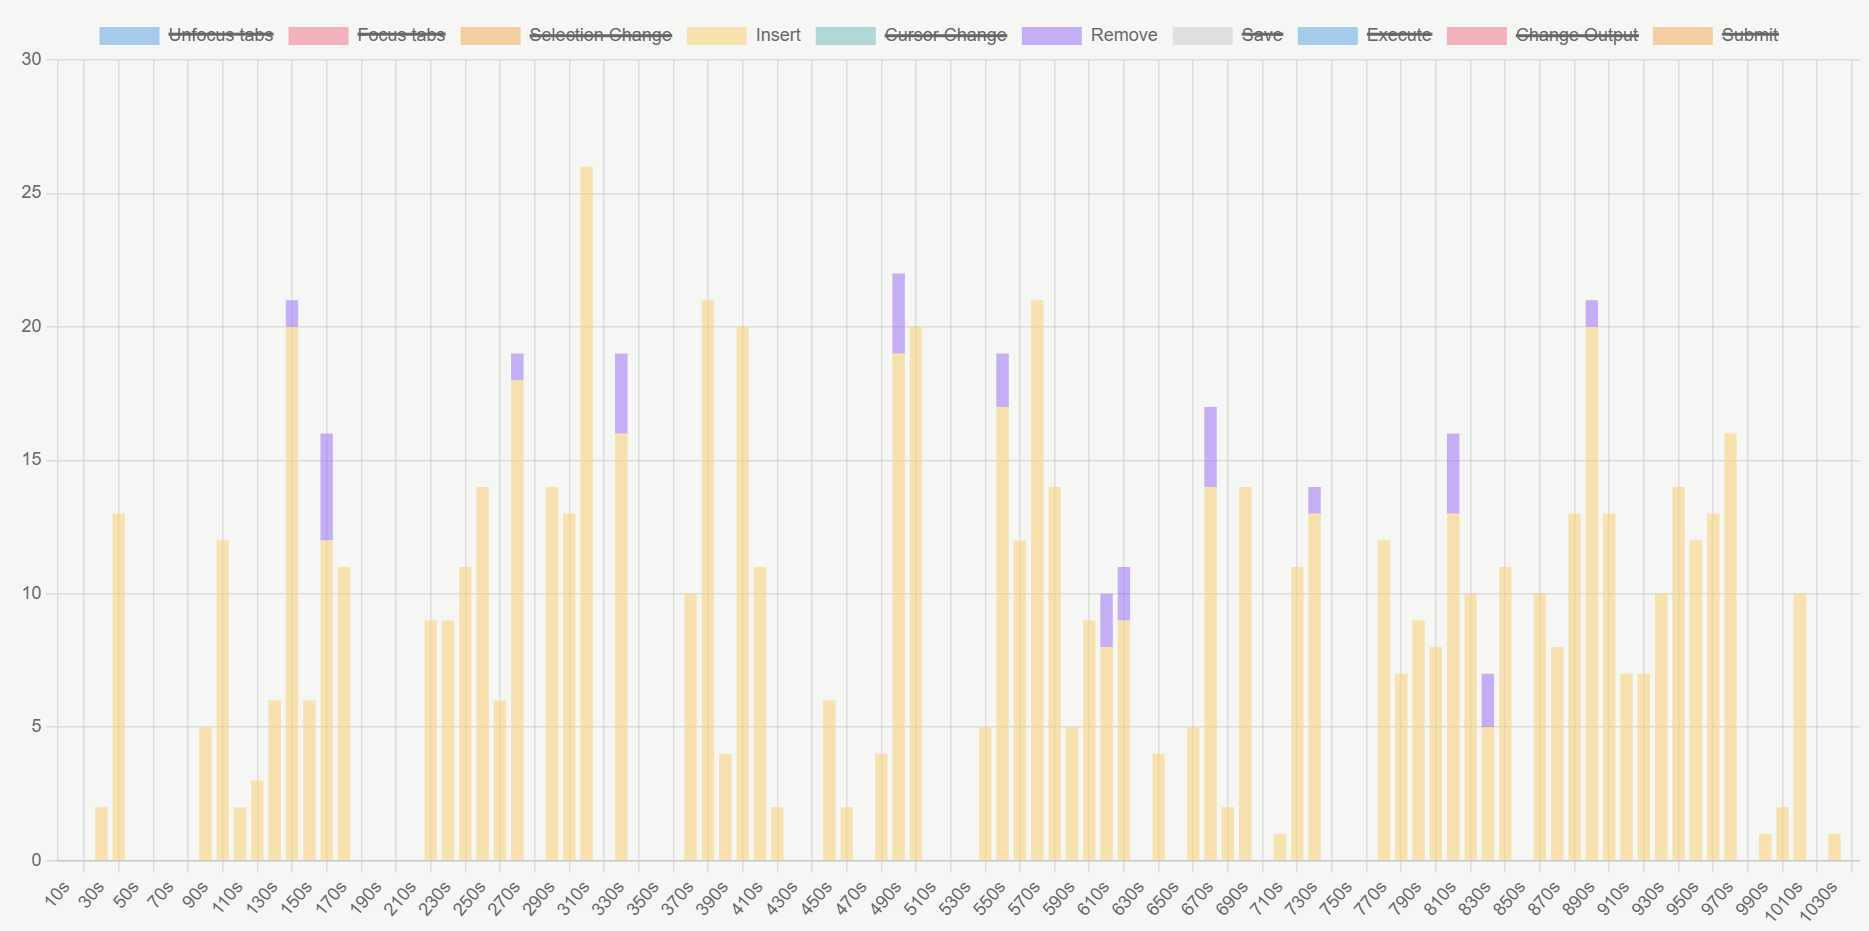
\includegraphics[width=0.49\textwidth]{experiment/insert-copy-ai.png}
        \caption{Bagan Histogram Perubahan Kode Program}
        \label{fig:5:2:3:rework}
    \end{figure}

    Pada Gambar \ref{fig:5:2:3:rework} sebelah kiri peserta mengerjakan dengan tidak melakukan kecurangan. Terjadi 1436 karakter yang dimasukkan dan 2240 karakter yang dihapus pada editor dengan total kode akhir memiliki panjang 362 karakter. Maka menggunakan rumus di atas, \textit{Code Churn Rate} pada peserta ini menjadi 10.15. Dengan nilai \textit{Code Churn Rate} yang tinggi maka peserta ini banyak mengubah kode program.
    
    Sebaliknya pada Gambar \ref{fig:5:2:3:rework} sebelah kanan peserta menggunakan AI untuk mengerjakan dengan men-\textit{copy} hasil kode AI ke dalam editor. Terjadi 1723 karakter yang dimasukkan dan 28 karakter yang dihapus pada editor dengan total kode akhir memiliki panjang 1771 karakter. Maka menggunakan rumus di atas, \textit{Code Churn Rate} pada peserta ini menjadi 0.99. Dengan nilai \textit{Code Churn Rate} yang rendah maka peserta ini tidak banyak mengubah kode program.

    Maka Pola Pergantian Kode ini dinilai dengan \textit{Code Churn Rate}, semakin tinggi nilai tersebut maka semakin tinggi juga perubahan kode yang terjadi. Jika banyak perubahan kode maka dimungkinkan bahwa peserta tidak melakukan kecurangan pada saat pengerjaan.

    \item Pola \textit{Debugging} \\
    Pola ini dapat dilihat pada \textit{events} \verb|editor.change|, \verb|editor.changeCursor|, \verb|editor.change|\\\verb|Selection|, \verb|editor_input.input|, dan \verb|editor_output.change|. Pengguna yang melakukan \textit{debugging} pada saat mengerjakan akan lebih sering mengubah kode pada lokasi yang sama. Gambar \ref{fig:5:2:3:heatmapchange} sebelah kiri menunjukkan bahwa frekuensi lebih tinggi akan berwarna lebih merah dan menandakan pola debugging pada posisi tertentu yang dapat dilihat karena terjadinya banyak perubahan pada posisi yang sama dibandingkan dengan Gambar \ref{fig:5:2:3:heatmapchange} sebelah kanan yang memiliki frekuensi maksimum 12 pada warna yang paling merah.

    \begin{figure}[H]
        \centering
        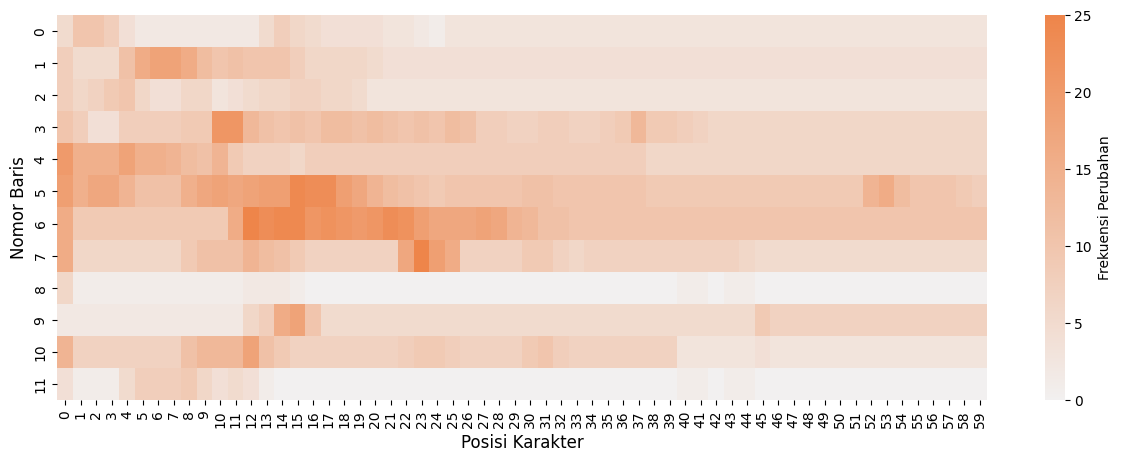
\includegraphics[width=0.49\textwidth]{experiment/change-heatmap.png}
        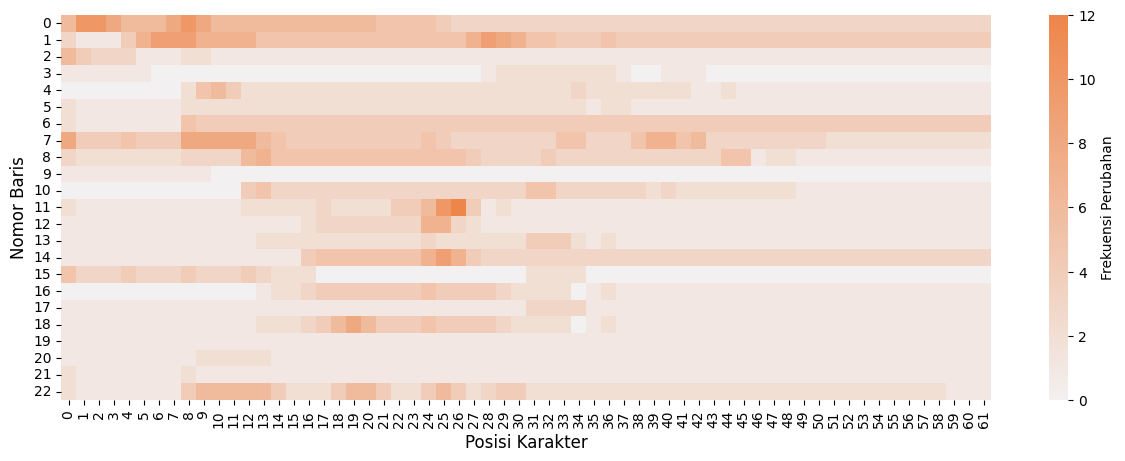
\includegraphics[width=0.49\textwidth]{experiment/change-heatmap-nodebug.png}
        \caption{Bagan Heatmap Perubahan Lokasi Kode Program}
        \label{fig:5:2:3:heatmapchange}
    \end{figure}
    
    Peserta yang \textit{debugging} juga akan mencoba untuk mengubah input dan melakukan aksi \textit{Execute} lebih banyak dibandingkan dengan peserta yang tidak melakukan \textit{debugging} pada saat mengerjakan soal. Gambar \ref{fig:5:2:3:debug} sebelah kiri menunjukkan warna kuning sebagai perubahan input dan warna biru sebagai aksi \textit{Execute} yang dilakukan sedangkan Gambar \ref{fig:5:2:3:debug} sebelah kanan menunjukkan warna biru sebagai perubahan input dan warna merah sebagai aksi \textit{Execute} yang dilakukan. Perbedaan kedua bagan adalah frekuensi dimana aksi \textit{Execute} dilakukan dan juga perubahan input. Maka pola \textit{debugging} juga dapat dilihat melalui frekuensi aksi \textit{Execute} dan juga frekuensi perubahan input.

    \begin{figure}[H]
        \centering
        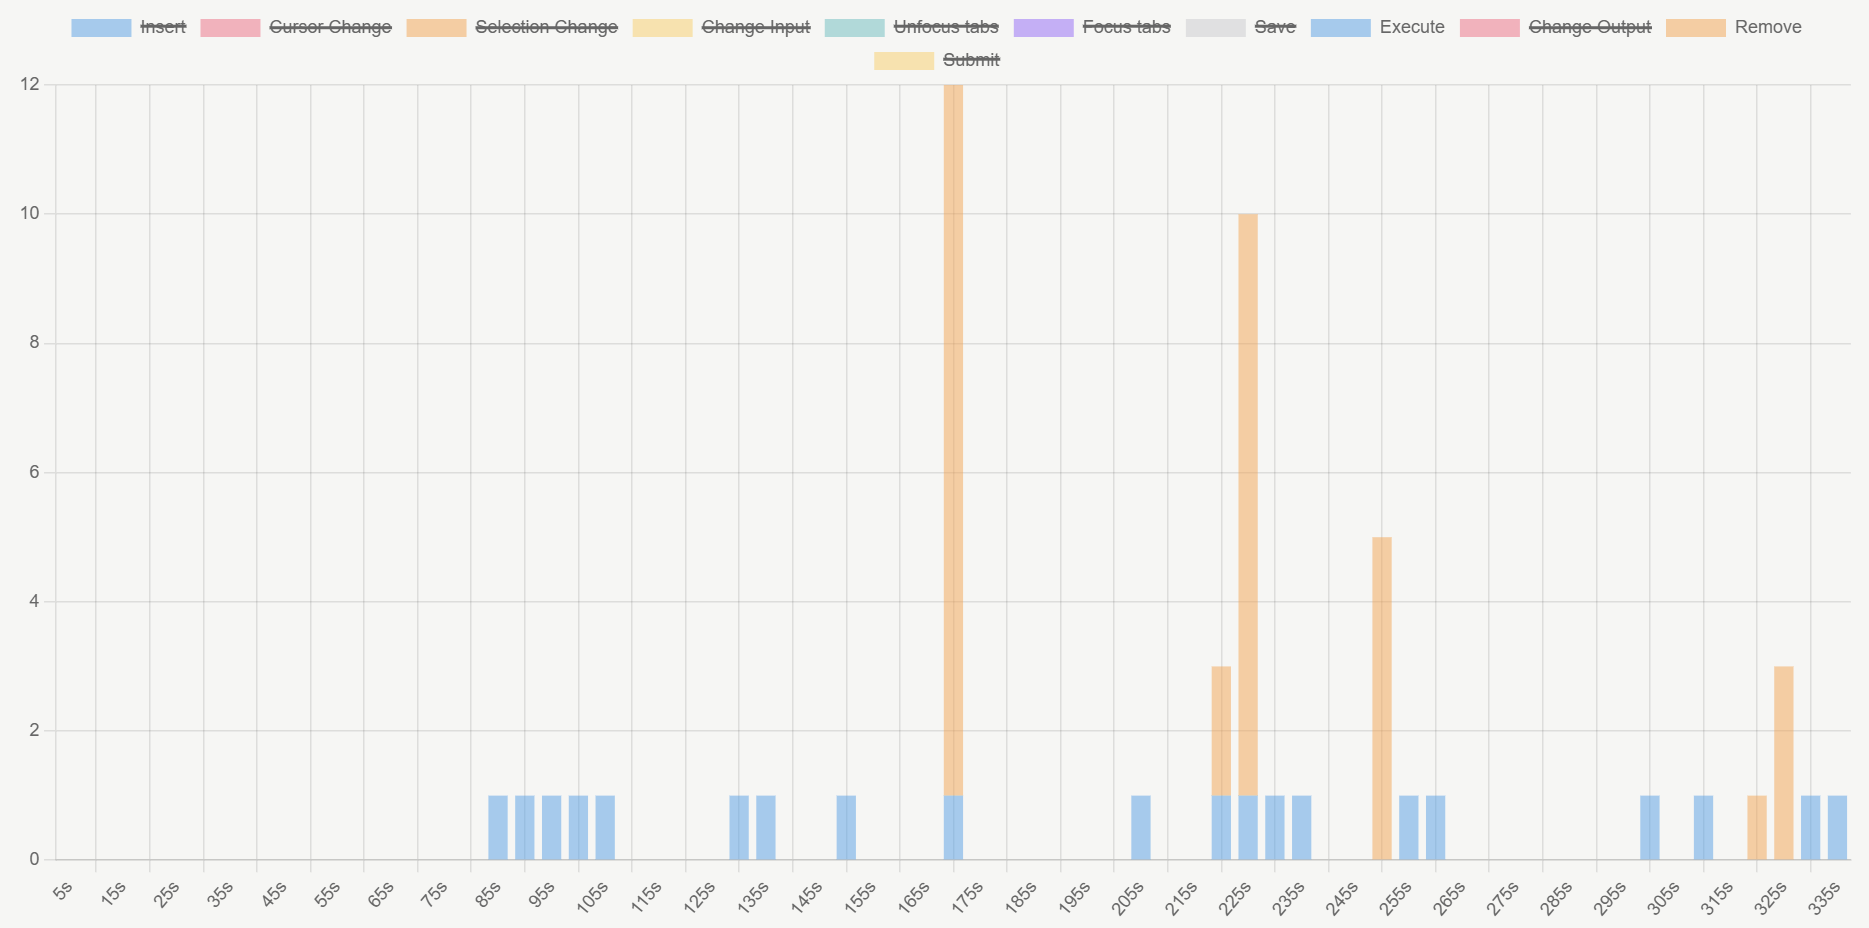
\includegraphics[width=0.49\textwidth]{experiment/debugging-many-io.png}
        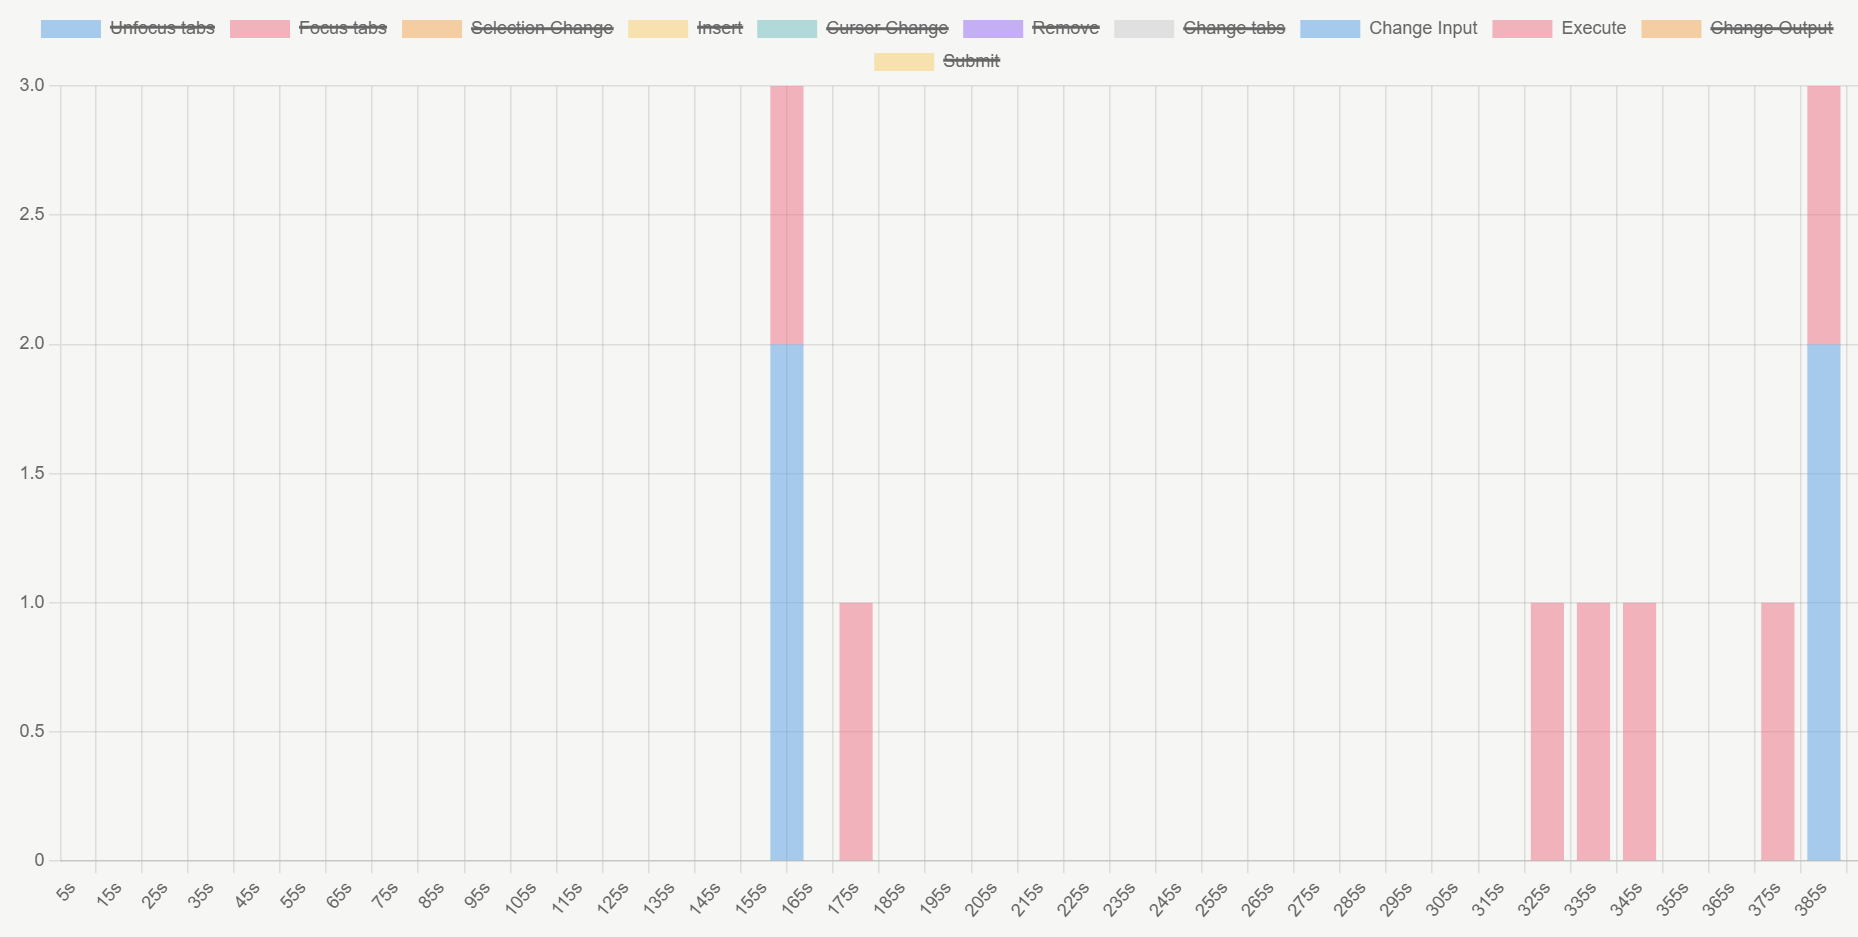
\includegraphics[width=0.49\textwidth]{experiment/debugging-less-io.png}
        \caption{Bagan Histogram Perubahan Input dan Aksi \textit{Execute}}
        \label{fig:5:2:3:debug}
    \end{figure}

    Pola \textit{Debugging} ini mendukung Pola Pergantian Kode untuk mengetahui apakah peserta melakukan kecurangan. Tetapi tidak dapat mengetahui pasti peserta yang melakukan kecurangan.

    \item Pola Perubahan Navigasi \\
    Pola ini dapat terlihat pada \textit{events} \verb|window.focus|, \verb|window.blur|, dan \verb|window.visibility|\\\verb|change|. Pola ini dilihat dengan membandingkan seberapa sering pengguna mengubah navigasi dalam sesi mengerjakan kode program. 
    Gambar \ref{fig:5:2:3:navigation} menunjukkan perbedaan bagan histrogram \textit{event} \verb|window.focus|, \verb|window.blur|, dan \verb|window.visibilitychange| pada peserta yang men-\textit{copy} kode program dari jawaban \textit{online} pada saat mengerjakan soal dan peserta yang mengerjakan soal hanya pada website SharIF Judge.  

    \begin{figure}[H]
        \centering
        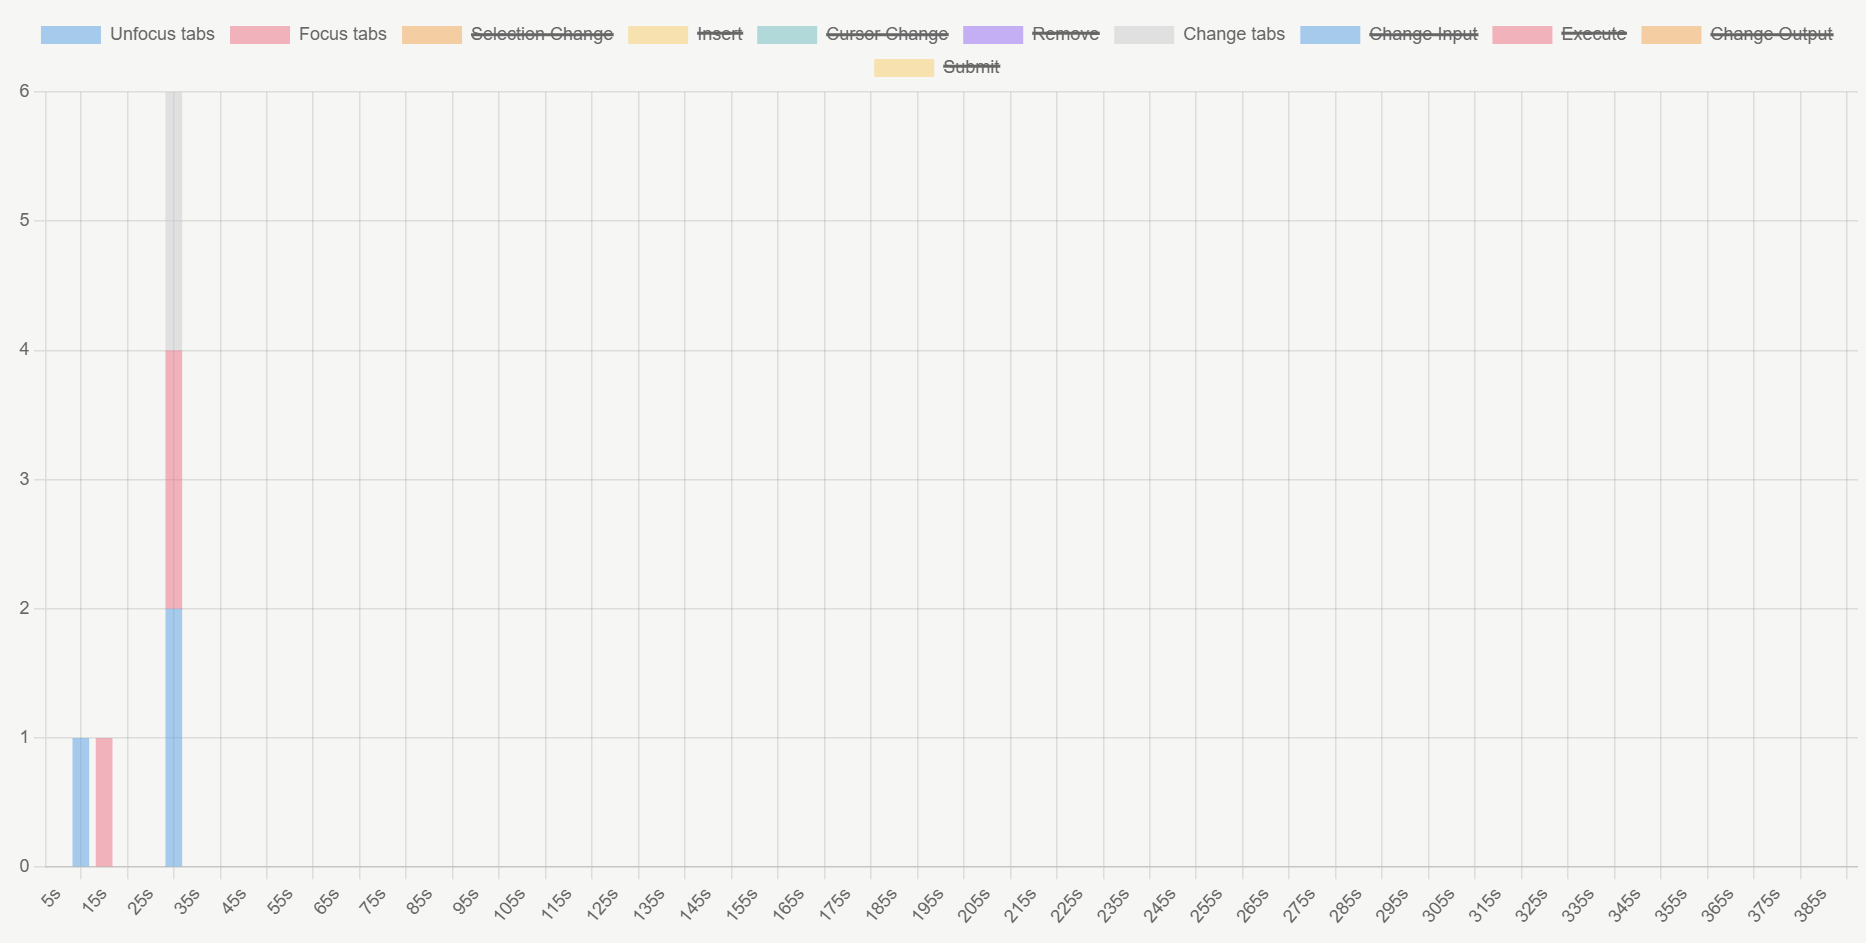
\includegraphics[width=0.49\textwidth]{experiment/less-navigation.png}
        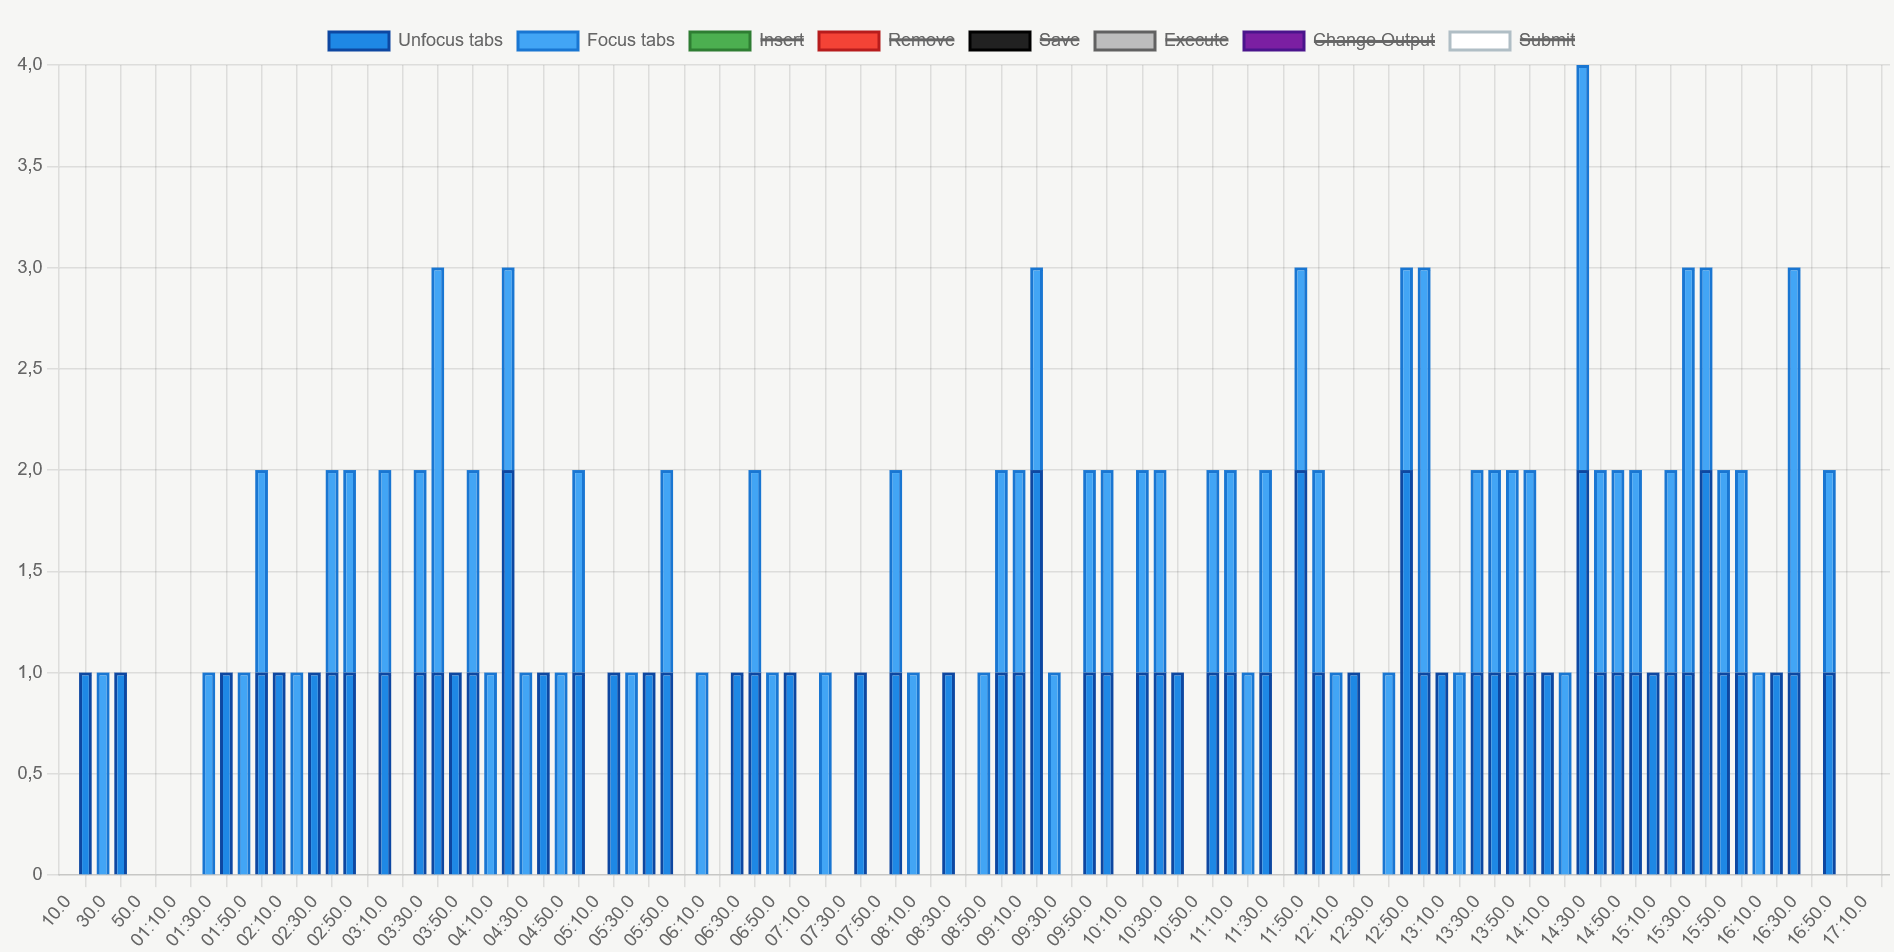
\includegraphics[width=0.49\textwidth]{experiment/many-navigation.png}
        \caption{Bagan Histogram Perubahan Navigasi}
        \label{fig:5:2:3:navigation}
    \end{figure}

    Pola Perubahan Navigasi dapat diukur dengan membatasi perubahan \textit{event} tersebut dalam waktu tertentu. Jika nilai melebihi batas, maka peserta dapat diduga melakukan kecurangan.

    \item Pola Berpikir \\
    Pola ini dapat dilihat pada keseluruhan \textit{events} yang terjadi. Pada Pola ini dapat dilihat dari saat pemberhentian peserta sebelum melakukan perubahan yang kompleks terhadap kode program dan juga keseringannya terjadinya pemberhentian.
    
    \begin{figure}
        \centering
        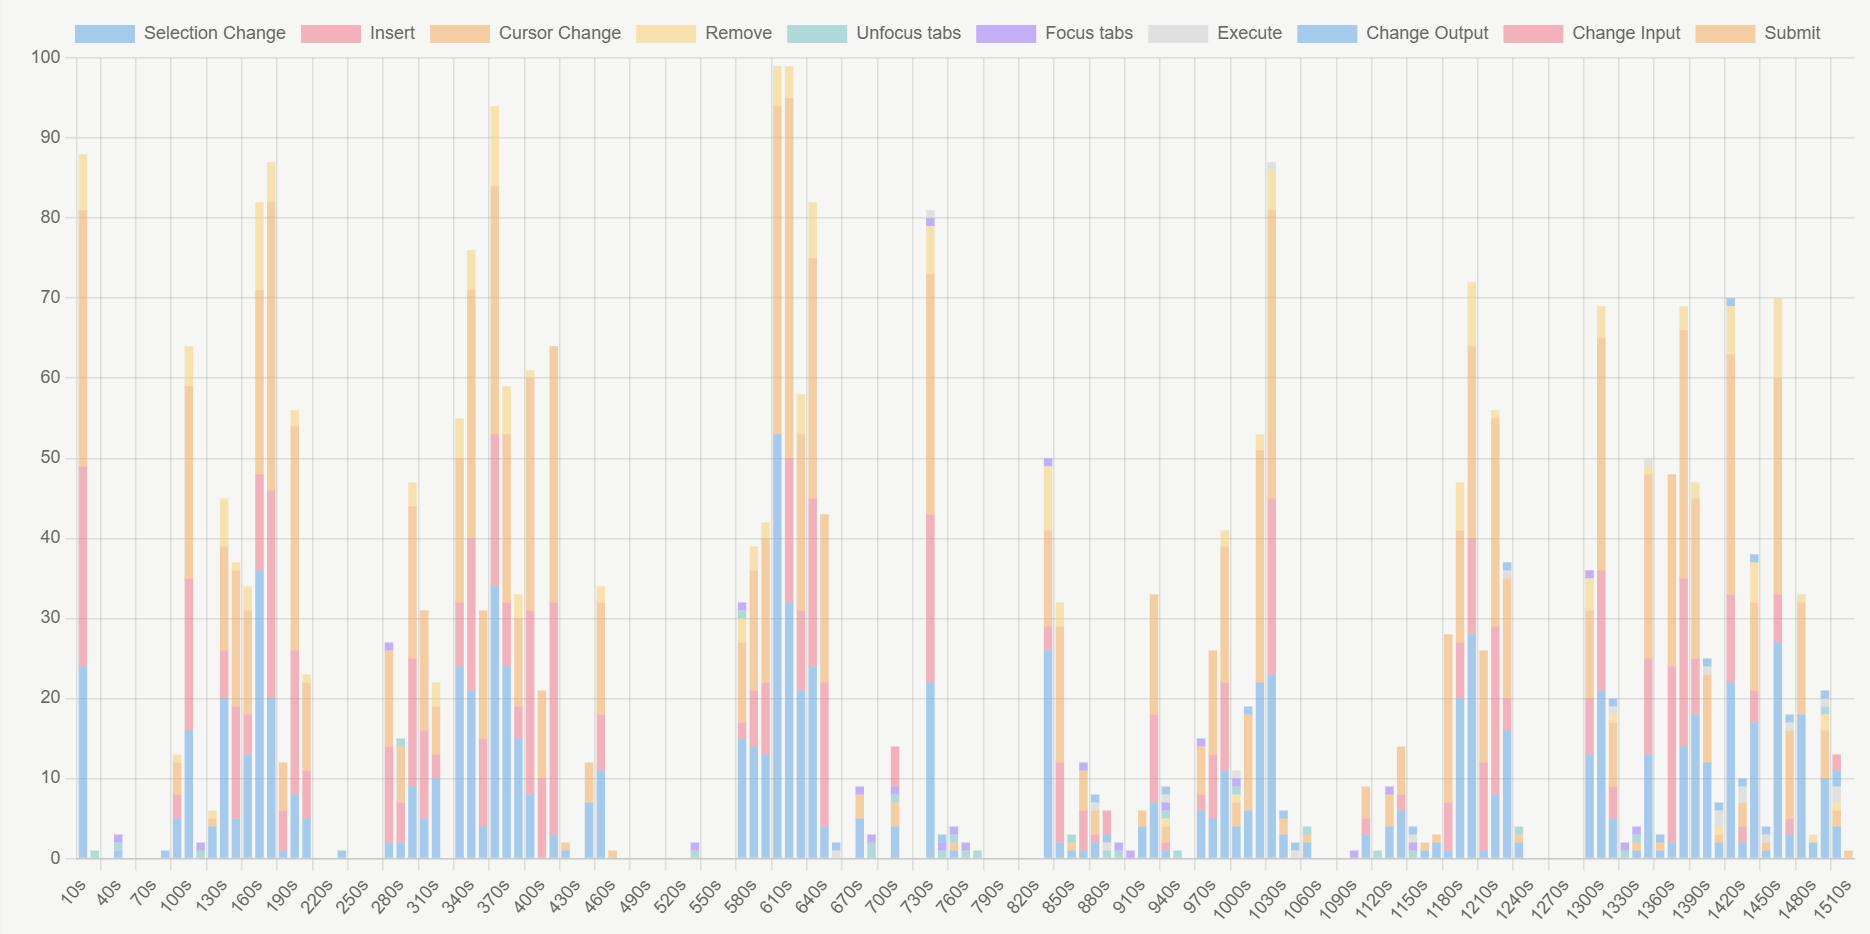
\includegraphics[width=\textwidth]{experiment/berpikir-2.png}
        \caption{Bagan Histogram Perubahan}
        \label{fig:5:2:3:berpikir}
    \end{figure}

    \begin{figure}
        \centering
        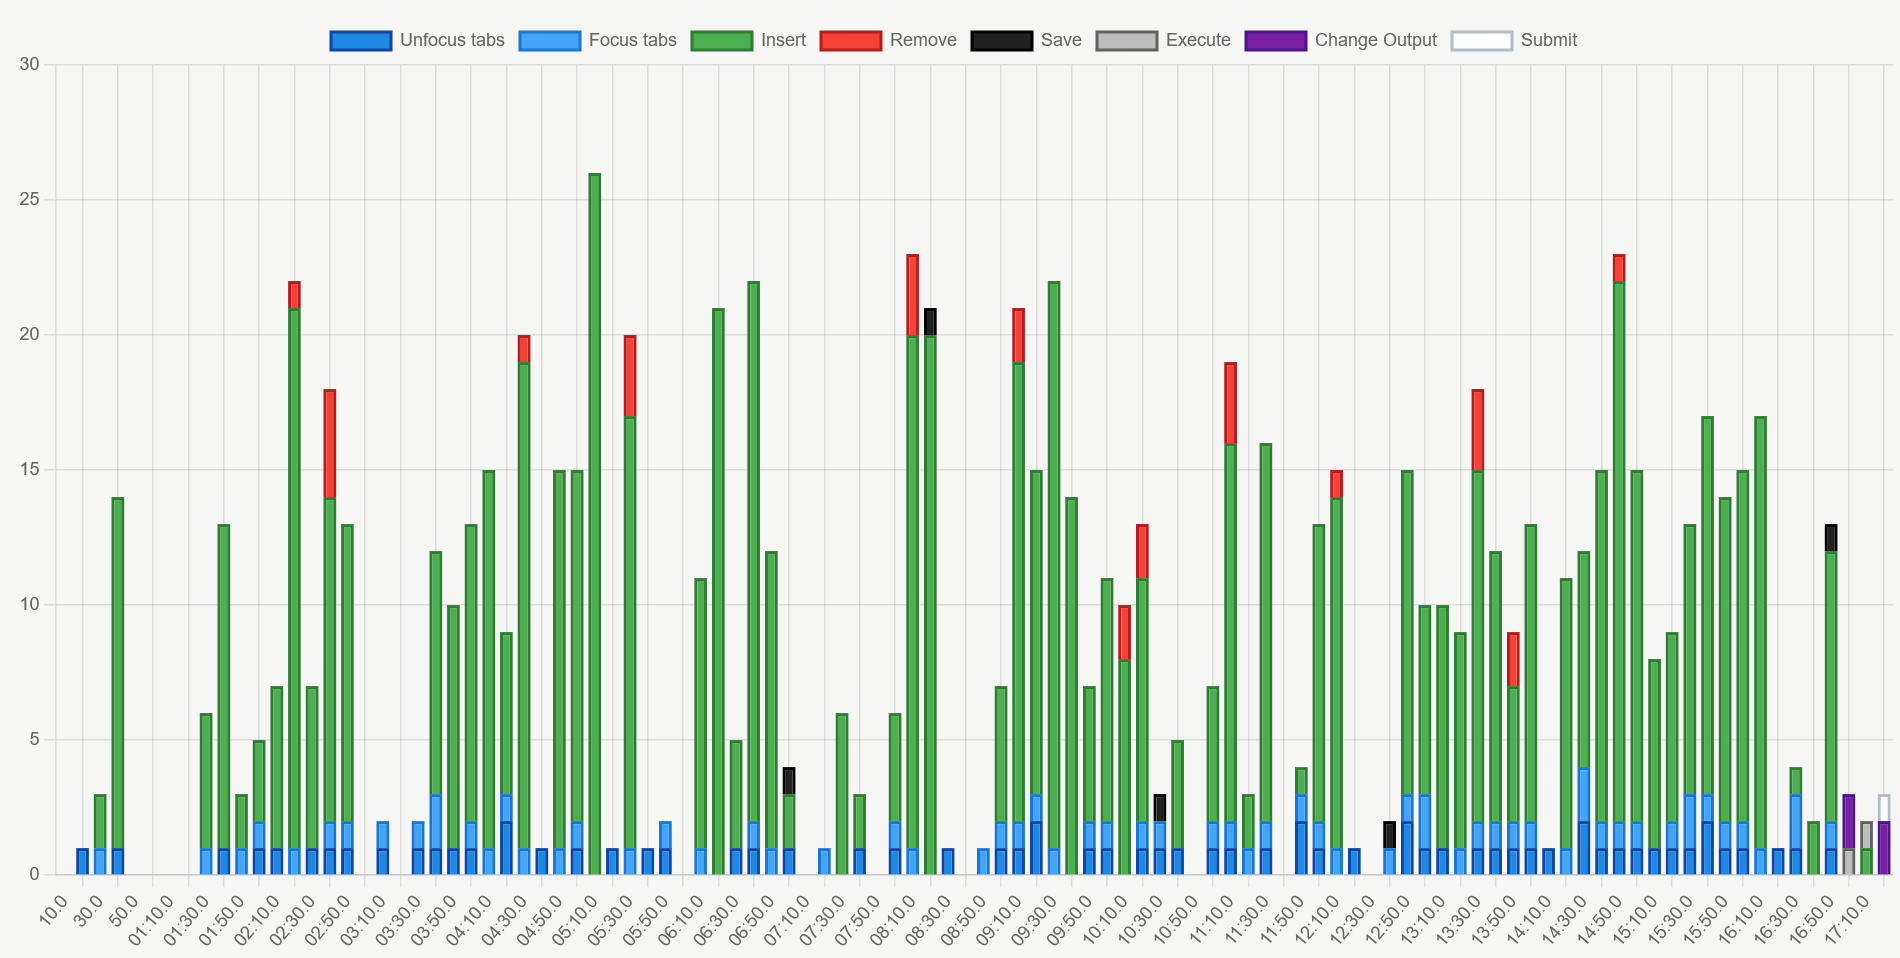
\includegraphics[width=\textwidth]{experiment/non-berpikir.png}
        \caption{Bagan Histogram Perubahan}
        \label{fig:5:2:3:tidakberpikir}
    \end{figure}

    Gambar \ref{fig:5:2:3:berpikir} memiliki histogram yang dipisah setiap sepuluh detik dan memiliki waktu yang cukup lama sebelum melakukan perubahan yang cukup besar. Sebaliknya Gambar \ref{fig:5:2:3:tidakberpikir} menunjukkan peserta yang men-\textit{copy} kode dari sumber jawaban \textit{online}. Bagan ini menunjukkan lebih seringnya berhenti untuk melihat jawaban terlebih dahulu dan durasi pemberhentiannya lebih kecil dibandingkan bagan histogram pertama.

    Pola ini dinilai dengan memberikan batas frekuensi berpikir dan lamanya berpikir dalam suatu waktu. Jika nilai melebihi batas, maka peserta dapat diduga melakukan kecurangan.

    \newpage
    
    \item Pola \textit{Copy-Paste} \\
    Pola ini merupakan pola sederhana dimana jika terjadinya penambahan kode yang panjang atau besar tetapi tidak melakukan penghapusan yang panjang atau besar terlebih dahulu, maka akan diduga melakukan kecurangan.

\end{itemize}

Tetapi pola-pola tersebut dapat juga mendapatkan \textit{false positive} karena banyaknya \textit{variable} yang harus diperhatikan dalam menentukan tidakan kecurangan itu sendiri. \textit{Variable} yang dimaksudkan antara lain adalah kesulitan masalah dan pengalaman programing. Jika kesulitan masalah mudah maka peserta dapat mengerjakan dengan mudah dan tidak memerlukannya \textit{debugging}, begitu juga jika pengalaman programing yang tinggi.